% !TEX root = main.tex

\section{微积分的应用}
这一章其实最关键的是建模,即如何用微元的思想对具体问题进行刻画. 至于具体的积分计算,则是第\ref{sec:indefinite_integration}章、第\ref{sec:definite_integration}章的内容.
\subsection{面积}
\begin{enumerate}
	\item 直角坐标
	\[\diff A=y\diff x=(f(x)-g(x))\diff x\]
	积分上下限即两曲线端点
	\item 参数方程$(x(t),y(t)),t\in[\alpha,\beta]$(简单闭曲线$\Gamma$,端点相连$x(\alpha)=x(\beta),y(\alpha)=y(\beta)$,其他地方不相交\footnote{规定曲线的正向:沿着曲线的正向走,其包围的有界区域始终在曲线左侧})
	\[\diff A=y(t)\diff x(t)\implies A=\textcolor{red}{-}\oint_\Gamma y\diff x\]
	积分上下限为$\alpha,\beta$
	\item 极坐标(曲线$r(\theta)$与向径$\theta=\alpha,\theta=\beta$所围成的区域)
	\[\diff A=\dfrac{1}{2}r^2(\theta)\diff\theta\]
	积分上下限为$\alpha,\beta$
\end{enumerate}
\begin{example}
求$r=3\cos\theta$和$r=1+\cos\theta$所围公共部分的面积
\end{example}
\begin{analysis}
两条曲线如下图所示,黄色部分即为要求的面积.
\begin{center}
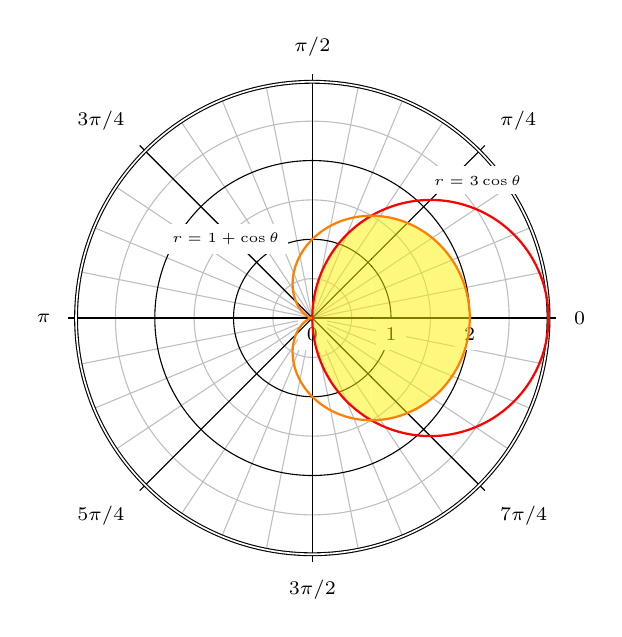
\begin{tikzpicture}
% Draw the lines at multiples of pi/12
\foreach \ang in {0,...,31} {
  \draw [lightgray] (0,0) -- (\ang * 180 / 16:3);
}

% Concentric circles and radius labels
\foreach \s in {0, 1, 2} {
  \draw [lightgray] (0,0) circle (\s + 0.5);
  \draw (0,0) circle (\s);
  \node [fill=white] at (\s, 0) [below] {\scriptsize $\s$};
}

% Add the labels at multiples of pi/4
\foreach \ang/\lab/\dir in {
  0/0/right,
  1/{\pi/4}/{above right},
  2/{\pi/2}/above,
  3/{3\pi/4}/{above left},
  4/{\pi}/left,
  5/{5\pi/4}/{below left},
  7/{7\pi/4}/{below right},
  6/{3\pi/2}/below} {
  \draw (0,0) -- (\ang * 180 / 4:3.1);
  \node [fill=white] at (\ang * 180 / 4:3.2) [\dir] {\scriptsize $\lab$};
}

% The double-lined circle around the whole diagram
\draw [style=double] (0,0) circle (3);

\fill [fill=yellow, opacity=0.5, samples=200] plot [domain=pi/3:2*pi/3]
	(xy polar cs:angle=\x r, radius= {3*cos(\x r)});
\draw [thick, color=red, domain=0:2*pi, samples=200, smooth]
	plot (xy polar cs:angle=\x r, radius={3*cos(\x r)});
\fill [fill=yellow, opacity=0.5, samples=200] plot [domain=-pi/3:pi/3]
	(xy polar cs:angle=\x r, radius= {1+cos(\x r)});
\draw [thick, color=orange, domain=0:2*pi, samples=200, smooth]
	plot (xy polar cs:angle=\x r, radius={1+cos(\x r)});
\node [fill=white] at (2.1,1.75) {\tiny $r=3\cos \theta$};
\node [fill=white] at (-1.1,1) {\tiny $r=1+\cos \theta$};
\end{tikzpicture}
\end{center}
\par 注意在实际解题过程中,并没有图画作为辅助,因此需要自己判断积分区间.
\par 首先求定义域.
\[r\geq 0 \implies \theta\in[-\dfrac{\pi}{2},\dfrac{\pi}{2}]\]
\par 其次求出两曲线交点.
\[r=1+\cos\theta=3\cos\theta\implies\theta=\pm\dfrac{\pi}{3}\]
\par 判断对称性.
由于$\cos\theta$为偶函数,故两曲线都关于极轴对称.
\par 考虑内外关系,对小极径所在曲线进行积分.
\[A=2\cdot\dfrac{1}{2}\lrp{\intabu{0}{\frac{\pi}{3}}{(1+\cos\theta)^2}{\theta}+\intabu{\frac{\pi}{3}}{\frac{\pi}{2}}{(3\cos\theta)^2}{\theta}}=\dfrac{5}{4}\pi\]
\end{analysis}
\par 如果是单一极坐标曲线求面积,则一般关注其最大最小极径以及其对称性.

\subsection{体积}
\begin{enumerate}
	\item 旋转体(不是绕$x$轴、$y$轴旋转,则先做一个平移)
\[\diff V=\pi[f(x)]^2\diff x\]
	\item 已知截面积
\[\diff V=A(x)\diff x\]
\end{enumerate}

\subsection{弧长}
\begin{center}
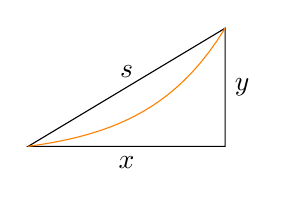
\begin{tikzpicture}[domain=0:2.5]
\draw (0,0) --node[below] {$\diff x$} (2.5,0) --node[right] {$\diff y$} (2.5,1.5) --node[left,above] {$\diff s$} cycle;
\draw[color=orange] plot (\x,{1.5/(exp(2.5)-1)*(exp(\x)-1)});
\end{tikzpicture}
\end{center}
\[\diff s=\sqrt{\diff x^2+\diff y^2}=\sqrt{1+\lrp{\dfrac{\diff y}{\diff x}}^2}\diff x\]
\begin{enumerate}
	\item 直角坐标
	\[\diff s^2=(1+[f'(x)]^2)\diff x^2\]
	\item 参数方程
	\[\diff s^2=([x(t)]^2+[y(t)]^2)\diff t^2\]
	\item 极坐标(通过$x=r\cos\theta,y=r\sin\theta$转直角坐标推导)
	\[\diff s^2=r^2\diff\theta^2+\diff r^2\]
\end{enumerate}

\subsection{曲率}
\begin{definition}[曲率]
用切线夹角与弧长之比来衡量曲线的弯曲程度,即
\[K=\left|\dfrac{\diff\varphi}{\diff s}\right|\]
\end{definition}
\begin{enumerate}
	\item 直角坐标
	\[K=\dfrac{|y''|}{(1+y'^2)^\frac{3}{2}}\]
	\item 参数方程(由参方推其他两个)
	\[K=\dfrac{|y''x'-y'x''|}{(x'^2+y'^2)^\frac{3}{2}}\]
	\item 极坐标
	\[K=\dfrac{|r^2+2r'^2-rr''|}{(r^2+r'^2)^\frac{3}{2}}\]
\end{enumerate}

\subsection{表面积}
旋转体的表面积可以通过以下的微元公式得到
\[\diff S=2\pi y\diff s\]
\par 注意想清楚取多少部分进行旋转,如上式的$y$仅仅是坐标轴一侧的$y$.
\begin{example}
求椭圆$\dfrac{x^2}{a^2}+\dfrac{y^2}{b^2}=1$绕$x$轴旋转所得旋转体的表面积
\end{example}
% http://www.nabla.hr/CL-DefiniteIntAppl5.htm
\begin{analysis}
本题解题方法来源于\footnote{Math StackExchange - How to Find the Surface Area of Revolution of An Ellipsoid from Ellipse Rotating, \url{https://math.stackexchange.com/questions/1379341}}.
对椭圆隐函数求导得
\[\frac{2x\diff x}{a^2} + \frac{2y\diff y}{b^2} = 0\]
故
\[\diff s = \sqrt{1 + (\frac{\diff y}{\diff x})^2}\diff x = \frac{1}{a^2}\,\frac{\diff x}{y}\,\sqrt{b^4x^2 + a^4y^2}\]
进而
\[\diff S = 2\pi y\diff s=2\pi \frac{1}{a^2}\,\sqrt{b^4x^2 + a^4y^2}\diff x\]
两边进行积分有
\[S = 2\frac{2\pi}{a^2}\int_{0}^{a} \sqrt{b^4x^2 + a^4y^2}\diff x\]
将
\[y^2 = b^2 - \frac{b^2}{a^2}\,x^2\]
代入有
\[S = 4\pi\,\frac{b}{a}\int_{0}^{a} \sqrt{a^2 - \varepsilon^2x^2}\diff x\]
其中,$\varepsilon^2=\sqrt{a^2-b^2}\Big/a^2$为椭圆离心率的平方,参数方程$x=a\sin\theta$
\[S = 4\pi\,ab\,\int_{0}^{\frac{\pi}{2}} \sqrt{1 - \varepsilon^2\sin^2\theta}\,\cos\theta\diff\theta\]
三角代换,令$\sin\phi = \varepsilon\sin\theta$,则$\cos\phi\diff\phi = \varepsilon\cos\theta\diff\theta$,故
\[S = 4\pi\,\frac{ab}{\varepsilon}\,\int\cos^2\phi\diff\phi\]
直接对其积分即可,将结果逐步回代得
\[S = 
2\pi\,\frac{ab}{\varepsilon}\lrp{\arcsin(\varepsilon) + \varepsilon\,\frac{b}{a}}= 
2\pi\,b^2\lrp{1 + \frac{a}{b}\,\frac{\arcsin(\varepsilon)}{\varepsilon}}\]
\end{analysis}

\subsection{质心}
\begin{theorem}[古鲁金(Guldin)第一定理]
质量分布均匀的平面曲线弧的质心坐标$(\bar{x},\bar{y})$由下式得出
\[2\pi\bar{x}l=S_1\qquad 2\pi\bar{y}l=S_2\]
其中,$S_1$和$S_2$分别为曲线弧绕$y$轴和绕$x$轴所得旋转体的侧面积,$l$为弧长.
\end{theorem}
其基本思想即将旋转体的侧面积转化为圆柱的侧面积.
\begin{theorem}[古鲁金第二定理]
质量分布均匀的平面图形绕此平面上一条与之不相交的直线旋转,所得旋转体的体积由下式给出
\[V=2\pi\bar{y}S\]
\end{theorem}